%yright 2007, 2008, 2009 Elsevier Ltd
%% 
%% This file is part of the 'Elsarticle Bundle'.
%% ---------------------------------------------
%% 
%% It may be distributed under the conditions of the LaTeX Project Public
%% License, either version 1.2 of this license or (at your option) any
%% later version.  The latest version of this license is in
%%    http://www.latex-project.org/lppl.txt
%% and version 1.2 or later is part of all distributions of LaTeX
%% version 1999/12/01 or later.
%% 
%% The list of all files belonging to the 'Elsarticle Bundle' is
%% given in the file `manifest.txt'.
%% 

%% Template article for Elsevier's document class `elsarticle'
%% with numbered style bibliographic references
%% SP 2008/03/01

% \documentclass[preprint,11pt]{elsarticle}
\documentclass[final,1p,12pt]{elsarticle}

%\documentclass[final,1p,times]{elsarticle}


%% Use the option review to obtain double line spacing
%%\documentclass[authoryear,preprint,review,12pt]{elsarticle}

%% Use the options 1p,twocolumn; 3p; 3p,twocolumn; 5p; or 5p,twocolumn
%% for a journal layout:
%% \documentclass[final,1p,times]{elsarticle}
%% \documentclass[final,1p,times,twocolumn]{elsarticle}
%% \documentclass[final,3p,times]{elsarticle}
%% \documentclass[final,3p,times,twocolumn]{elsarticle}
%% \documentclass[final,5p,times]{elsarticle}
%% \documentclass[final,5p,times,twocolumn]{elsarticle}

%%% For including figures, graphicx.sty has been loaded in
%% elsarticle.cls. If you prefer to use the old commands
%% please give \usepackage{epsfig}


\usepackage{epsfig}
%\usepackage{cite}
%\usepackage{mcite}
\usepackage{array,tabularx,epsfig,mathrsfs,graphicx,rotating}
\usepackage{ifthen}
\usepackage{amsfonts}
\usepackage{ragged2e}
\PassOptionsToPackage{hyphens}{url}
\usepackage[hyphens]{url}
\usepackage{hyperref}
\usepackage{listings}
\usepackage{lineno}
\usepackage{subfigure}
\usepackage{epstopdf}
% Custom colors
\usepackage{color}
\usepackage{float}
\usepackage{verbatim}
\usepackage{color,soul}

% to cross text
\usepackage[normalem]{ulem} % either use this (simple) or
\usepackage{soul} % use this (many fancier options)
\usepackage{amsmath,amssymb}

\let\originallesssim\lesssim
\let\originalgtrsim\gtrsim

\DeclareRobustCommand{\lesssim}{%
  \mathrel{\mathpalette\lowersim\originallesssim}%
}
\DeclareRobustCommand{\gtrsim}{%
  \mathrel{\mathpalette\lowersim\originalgtrsim}%
}

\makeatletter
\newcommand{\lowersim}[2]{%
  \sbox\z@{$#1<$}%
  \raisebox{-\dimexpr\height-\ht\z@}{$\m@th#1#2$}%
}
\makeatother


\hypersetup{
  colorlinks=true,
  linkcolor=blue,
  citecolor=blue,
  urlcolor=blue
}




\graphicspath{{figs/}}


\pdfinfo{
   /Author (Chekanov et al)
   /Title  (Studies of granularity of a hadronic calorimeter for tens-of-TeV jets  at a 100 TeV pp collider)
   /CreationDate (D:2017)
   /Subject (PDFLaTeX)
   /Keywords (PDF;LaTeX)
}


\textheight=22cm
\textwidth=14.5cm

\newcommand{\beq}{\begin{equation}}
\newcommand{\eeq}{\end{equation}}
\newcommand{\la}{\langle}
\newcommand{\promc}{{\sc ProMC}}
\newcommand{\ra}{\rangle}
\newcommand{\eps}{\epsilon}
\newcommand{\ud}{\mathrm{d}}
\newcommand{\Ec}{\mathcal{E}}
\newcommand{\Fc}{\mathcal{F}}
\newcommand{\Za}{\mathrm{Z_1}}
\newcommand{\Zb}{\mathrm{Z_2}}
\newcommand{\Zn}{\mathrm{Z_n}}
\newcommand{\F}{\mathrm{F}}

\chardef\til=126
\newcommand{\GEANTfour} {\textsc{geant4}}
\newcommand{\pythia} {\textsc{Pythia8~}}
\newcommand{\pt}{\ensuremath{p_{\mathrm{T}}}}


\journal{}

\begin{document}
%\hfill ANL-HEP-149528
\definecolor{mygreen}{rgb}{0,0.6,0} \definecolor{mygray}{rgb}{0.5,0.5,0.5} \definecolor{mymauve}{rgb}{0.58,0,0.82}

\lstset{ %
 backgroundcolor=\color{white},   % choose the background color; you must add \usepackage{color} or \usepackage{xcolor}
 basicstyle=\footnotesize,        % the size of the fonts that are used for the code
 breakatwhitespace=false,         % sets if automatic breaks should only happen at whitespace
 breaklines=true,                 % sets automatic line breaking
 captionpos=b,                    % sets the caption-position to bottom
 commentstyle=\color{mygreen},    % comment style
 deletekeywords={...},            % if you want to delete keywords from the given language
 escapeinside={\%*}{*)},          % if you want to add LaTeX within your code
 extendedchars=true,              % lets you use non-ASCII characters; for 8-bits encodings only, does not work with UTF-8
 keepspaces=true,                 % keeps spaces in text, useful for keeping indentation of code (possibly needs columns=flexible)
 frame=tb,
 keywordstyle=\color{blue},       % keyword style
 language=Python,                 % the language of the code
 otherkeywords={*,...},            % if you want to add more keywords to the set
 rulecolor=\color{black},         % if not set, the frame-color may be changed on line-breaks within not-black text (e.g. comments (green here))
 showspaces=false,                % show spaces everywhere adding particular underscores; it overrides 'showstringspaces'
 showstringspaces=false,          % underline spaces within strings only
 showtabs=false,                  % show tabs within strings adding particular underscores
 stepnumber=2,                    % the step between two line-numbers. If it's 1, each line will be numbered
 stringstyle=\color{mymauve},     % string literal style
 tabsize=2,                        % sets default tabsize to 2 spaces
 title=\lstname,                   % show the filename of files included with \lstinputlisting; also try caption instead of title
 numberstyle=\footnotesize,
 basicstyle=\small,
 basewidth={0.5em,0.5em}
}


\begin{frontmatter}

\title{Decoherent and its experiments}
%%%%%%%%%%%%%%%%%%%%%%%%%%%%%%%%%%%%%%%%%%%%%%%%%%%%%%%%%%%%%%%

\author[add3]{C.-H. Yeh}
\ead{a9510130375@gmail.com}



\address[add3]{
Department of Physics and Center for High Energy and High Field Physics, 
National Central University, Chung-Li, Taoyuan City 32001, Taiwan
}





\begin{abstract}
This documentary is used to describe several topics including the fundamental concepts of the decoherent, and some of the experiments related to it. The whole document is based on the knowledge I have dabbled and absorbed, and I'm trying to elaborate on the findings and opinions. If there exists some misunderstandings, please let me know. Actually the decoherence is the very new aspect for me to look at the quantum mechanism without applying the cord of the Copenhagen's interpretations, and it seems to be the very useful way in terms of fighting with some fundamental and philosophical questions happening in the Copenhagen's view. 
\end{abstract}

\begin{keyword}
decoherent, quantum entanglement, Copenhagen's interpretations, information
\end{keyword}
\end{frontmatter}
\tableofcontents



%%%%%%%%%%%%%%%%%%%%%%%%%%%%%%%%%%%%%%%%%%%%%%%%%%%%%%%%%%%%%%%%%%
\section{Introduction}
Over the decade, the class of the quantum mechanism has been being taught in the point of the Copenhagen's intetpretation\cite{Hollowood_2015}, which says the concept of the possibility is implanted in our world. In the form of the math, we can use the "wave function" to represent the intensity of the possibility happening this event. But till the recent year, upon the unsolved the problem raised by some of the physicists about the root of this possibility,  another party of the quantum mechanism came up for the fight! They applied the different way from the copenhagen's view,  which is using the superposition of the states to describe the events coming up, and after we conduct our measurement, the collapse of the wave function happening to the object(s) we would like to measure on is going to show up, and in the end, the state of the object will be fixed at the measured state, pointing to the concepts, "collapse". But the terrifying problem bothering us is that: How come the cat could be dead and alive at the same time in our daily life as an intuitive phenomenon?\\

Instead of ending up collapsing to the certain state at the final state, the new concept of the quantum mechanism: Decoherence, just heap up to the stage as the new comer going for the battle! The fundamental basis of this concept is very different from the copenhager's view as speaking of the final state. Actually in the point of view from decoherence, the superposition states won't collapse even if we can't measure them! And in perspective of this idea, many aspects of the quantum mechanism should be well-constructed again. Meanwhile, the multiple-world concept will be brought up as the production of the process.\\ 

In the short way of describing the concept of the decoherence, the "Environment-induced" system is the whole thing we can say sharply. Since the interaction between this quantum system and our macroscopic system happens, the coherence things which exists in the quantum system could be "destroyed" in the end by those "contamination" coming from the outer environment excluded by the quantum system, and it will end up demonstrating the properties acting like the classical way. The so-called "Decoherence" is the way we put the concept of "undermining the coherence things to be the decoherence one" into explaining the "collapse" in terms of the Copenhagen's interpretation but using the more general terminology to result in figuring out the more concrete way of confirming the logical deduction in the quantum mechanism.\\ 

In the following sections, at the first place, I will talk about the problems of the Copenhagen's view as the initiated topic since I think the items we have been being instilled is to apply that view to solve all of the problems happens in the quantum mechanism without mentioning another kinds of the paradigm elaborating on the quantum system without the "blinded" eye on the "non-measurable" observations. Second, I will move to the cord of the decoherence, which will be performed by the math writing in papers often and try to explain on them with the clear pictures. The third part will be the topics saying something related to the production of the decoherence. For instance, the quantum entanglement came up with the theory of the decoherence and the information transformation between two systems will be listed out in this section. In the end, the sorts of the experiment demonstrating the rationale of the decoherence will be written as the final section and then the conclusion for combining all topics above.\\

\section{The problem of the Copenhagen's interpretation}
From the rationale of the quantum theory comes from the Copenhagen's party, basically after our measurement has been conducted and the apparatus has already detected the real value of the observations, the state is fixed at the one we measure, and sort of the other states that appear in the apparatus which don't show up as our measurable states are abandoned eventually, and this will be the way we solve the "unsolvable"(at the moment)" puzzle and tackle those non-detectable states, and as we know, the party uses the way of extracting the measured state as our "collapse" state and describe that, the wave function at the beginning could show up with many kinds of the states mixed up together, and then evolving with the time in the space, ending up being caught up in our detector, and the states are collapsing into the "certain" cement state and won't change.\\ 

\subsection{The first puzzle- non-intuitive Superposition}
But is it right? In perspective of the experiment, it appears to be the right way to describe the wave function in this path. Nevertheless, in real life,  we can't see this sort of the "superposition state" as the example of the Schrodinger cat we've shown in the first section. So how can we find out this many-states composed wave function deductively instead of employing the hand-waving method - simply add them up to see is the first task.. This is the first aspect of the decoherence that can be utilized to solve the puzzle of the superposition stuff quoted in the view of the Copenhagen which was skipping this daunting issue.\\ 

\subsection{The second puzzle- Because you can't see, doesn't mean it, isn't there!}
Since the detector can only give us one value for the certain observation at a time, for example, we measure the electric field, and it will give us the certain measurable intensity of it with the evolving time causing the fluctuations.( Can do some averages or the threshold to select the one we want, and I will completely jump off the technic of measuring the value of it because of the theory of the quantum mechanism doesn't contain the detector being in capable of doing detecting something. ) So, intuitively, we could think of it as the certain state we get in the end, and carelessly, we just misunderstood it as the only state remains in the detector is the one we should pick up, and the other "mixed up" states that doesn't show up should be ignored as the background or nothing. Some experiments exhibit to us that the so-called "background" is non-negligible term even in the very big scale of astronomy stuff interact with the dust particles or other material floating in the space can happen the decoherence obviously!\cite{Kiefer}! And from the decoherence, we can quantitively say some of the real cases to be the evidence for us to rethink about this issue.\\

\subsection{The third puzzle- The uninterpreted possibility with the wave function}
As the textbook statement quoted from the point of Copenhagen's view, the square of the wave function, which is referring to the amplitude of the wave, means that the possibility of happening the given state. But the problem is: Where does it come from? Actually this is the transcendental term in their view, that means it is a kind of the presumptions and result in explaining most of our experiment well, but fundamentally there is no math or evidence to support this one philosophically. \\

Till there, the new thing is supposed to come out as the practical way to tackle this issue with adding the interaction between two systems, the one is the system included the measured system, the apparatus, and the other one is the environment. The so-called "Quantum Darwinism", which hears animated to me because of the Darwinism basically describes the interaction between the real nature and the life on earth, is the one can be the way of solving this issue by using the math skills taking the environment into account.\\  

In light of considering the interaction between the system of the interest and the environment is on the way, transferring the information between the two systems could be carrier out as the concepts of doing the interaction, and therefore, the "copied" information from the system to the environment should appear. Following this kind of the logic, the quantum entanglement, the many-world concepts will be released as the production of transferring the information.\\

\subsection{Let us get the benefit from the decoherence!}
Despite some of the puzzles remain unsolved even given a such good way to explain many puzzles in the Copenhagen's point as the theory of the decoherence, we can still look at the rest of the puzzles listed above solved by this theory. In the next section, the puzzles in the second section will be unraveled with the help of the decoherence, and also the math ( A little bit ) which is used to be the best way to say about the concepts directly, will also be listed as a way to describe the answer to the puzzles.\\

\section{What's "decoherence"?}
Be in charge of lightening the points of the decoherence\cite{joos1999elements} really solved the puzzles above, the first one thing to do is to describe the fundamental picture applied to tackle the problem. And after the well-defined rationale is nailed down certainly, then challenging the puzzles you've heard above and try to solve them with this new concepts is our very next step. \\
%%%%%%%%%%%%%%%%%%%%%%%%%%%%%%%%%%%%%%%%%%%%%%%%%%%%%%%%%%%%%%%%%%
\subsection{The infasturcture of the decoherence and its extension}
Actually, it is the very basic picture, that we just write down the real case we have in our real life without throwing away any possibility. Here is an example made by myself, when the certain particle with the certain state comes to our detector, and immediately puts the energy in it through some kinds of the interactions like the EM, and in a certain period of time depending on the resolution of the detector, you will get the certain state defined by the value you see on the panel of the detector. \\

Happily, you say "ok this is my final state" and turn in the value to your boss, then theoretically you just screw up the task from the point of the decoherence! (But experimentally you are right.XD) Because the value you measure is the one "dislocailzed" from the system, but not the case for the localized picture! In the real case with the localized picture, the states of the particle could remain the mixed up one, and we should consider them into account instead of kicking out them!  So, the foremost formula shown in the following line is the cord of the decoherence, which is used to say that the localized states will remain the same even we can't detect them ourselves:\\

And, since the environment will be taken into account, we should consider the effort of the environment as measuring the states by the detector, because the detector is connected with the environment unavoidably. And this will lead us to the new realm as the one I mentioned in the previous section, the information transferring will be the one of the most important processes when measuring the observations with the interaction between the system and environment. And since the decoherence, the same condition as the detector could happen in the environment:\\

With this so-called "system-environment interaction" version of the quantum system mapped out by the decoherence, much math supports the theory, even solves the puzzles we've told before deductively at the certain level of the assumption. 

\subsection{The math describing the basic decoherence}
I will take the example I make in the previous section to do the math process for clarifying the points clearly.\\

First of all, since the system of the quantum and the classical (macroscopic)  will be linked together as the total system for describing the decoherence, we need to have the description of the math on the correspondent between two systems, and the parameter of this one is so-called "the pointer state", which is necessary needed to be well-defined as the most important states. The math description is as follows:\\
\begin{equation}
| \varphi \rangle | \Phi \rangle \implies \sum_{\substack{
   m,n\\
  }} C_{mn} | \varphi_{n} \rangle | \Phi_{m} \rangle
\end{equation}
In this way of writing the definition of that means when we prepare the state at starting, and then we can do the measurement repeatably and result in the dynamics of the measurement interaction could be listed as the way we describe above. And later on, since the environment is involved in the interaction, the formula will be extended with acting the previous operator on the environment: \\
\begin{equation}
 (\sum_{\substack{
   m,n\\
  }} C_{mn} | \varphi_{n} \rangle | \Phi_{m} \rangle) | E_{0} \rangle \implies  
 ( \sum_{\substack{
  m,n\\
  }} C_{mn} | \varphi_{n} \rangle | \Phi_{m} \rangle | E_{n} )\rangle 
\end{equation}
So basically, the essence of the decoherence that is describing the interaction with the environment can be obtained from the formula. And we can draw the simplified pictures in Fig\ref{77777} to acknowledge this phenomenon more easily.\\

\begin{figure}
\begin{center}
   \subfigure[] {
   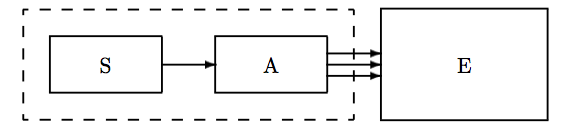
\includegraphics[width=0.6\textwidth]{7777.png}\hfill
   }
\end{center}
\caption{The figure illustrates the total system that we are considering in this report. The S means the signal of the interest, and the A means the detector we are using to detect the signal. The E is our cast that we are using this one to represent the interaction between the environment and the detector, which means that the classical environment influence the quantum system so much. }
\label{77777}
\end{figure}


Unfortunately, it's not so trivial as the formula say, just list the combinations of the total states with the possibility of all of them and end up doing it. Instead, the next step for us to proceed is to answer the extension question from there: How do we deal with those "non-measurable" observations and How do we describe the transition between this two system with some kinds of the transforming math. So the entanglement, the many-world idea could be extracted because of the idea for solving this problem.\\

\subsection{The vivid example for giving the explanation of the decoherence}
I make an example in this part for explaining the case more vivid. Please image that there is an atom popping up in the certain space, and from our basic knowledge, the energy of stimulating the electron from the ground state to the excited state can be calculated by the theory.( At there it doesn't matter where the excited state is I suppose. ). All of the sudden, we initiate sending the electromagnetic wave to the atom and subsequently, it will go through the back-and-forth processes of the excitation and emission. \\

Till now, the certain picture with the wave oscillating up and down that can be employed to describe the phase of the electron between 0 to $2\pi$ should show up in your mind. The case I'm talking now is so-called "Coherence" case since now the phase can be described as some of the combinations of the periodic waves. The picture attached in the Fig.\ref{9999} is applied to see this wave. ( At there the coherence is the same as the basic case of the coherence light, the same frequency of the wave. ), and in this case, the Schrodiger's cat stating at the dead and alive can be portrayed as this kinds of the pictures in the representative of the wave.\\ 

\begin{figure}
\begin{center}
   \subfigure[] {
   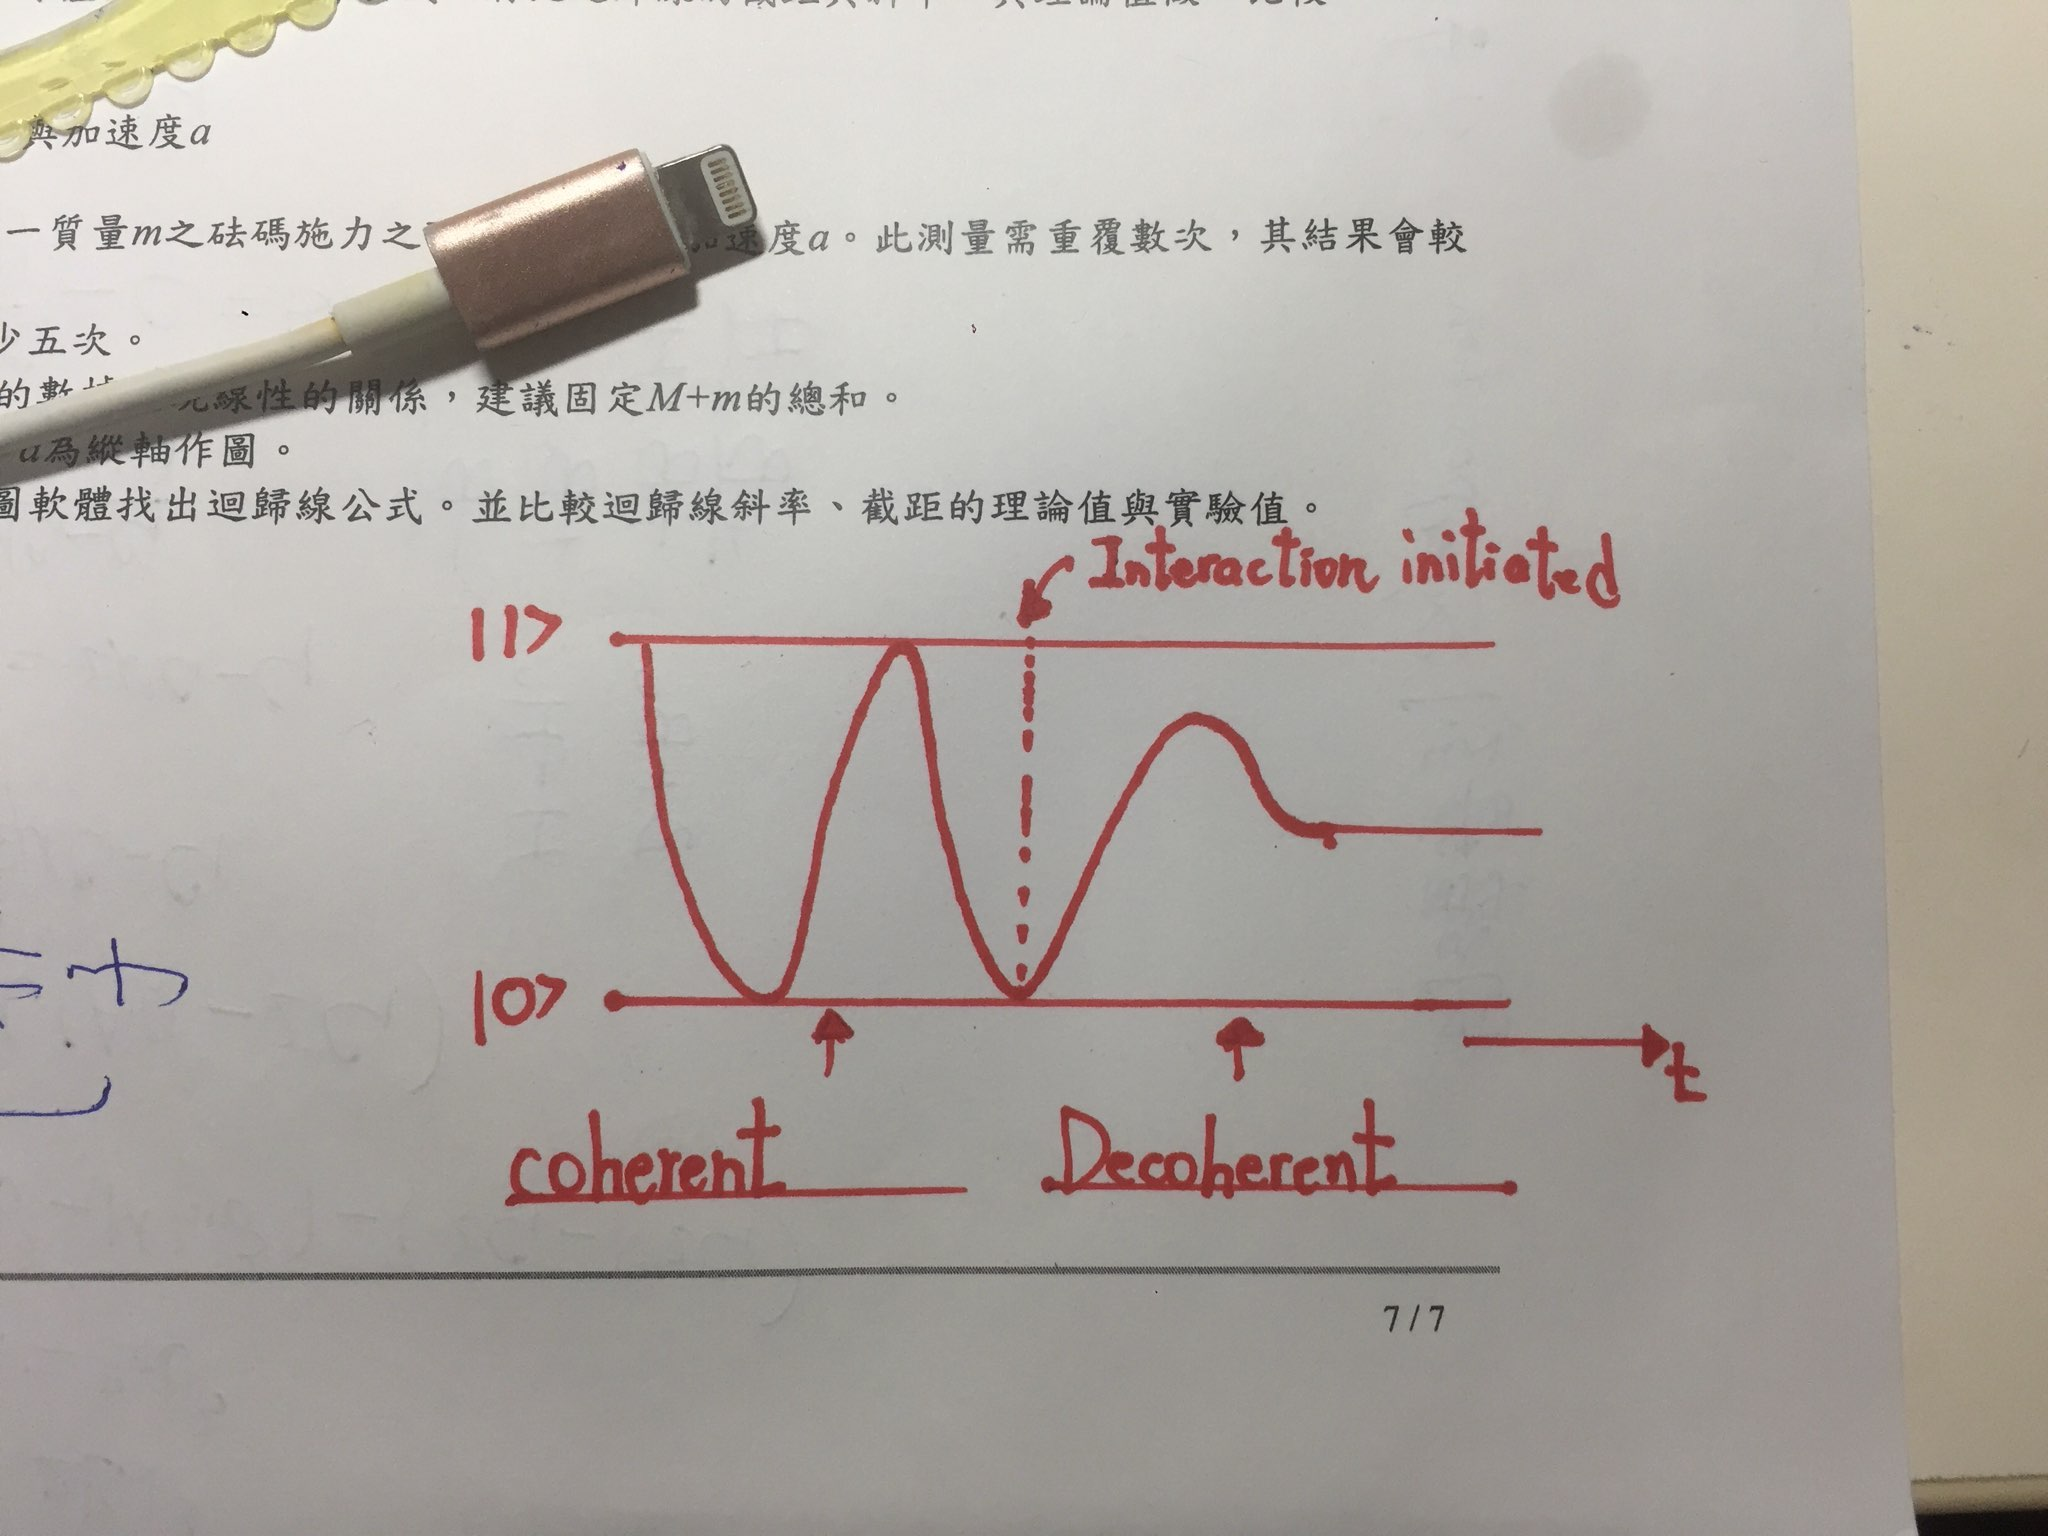
\includegraphics[width=0.8\textwidth]{E71B0522-CB89-4D9F-B3AA-A9FC2E2CEBA8.jpg}\hfill
   }
\end{center}
\caption{The figure illustrates the process of the decoherence. The transition within the two regions are shown in the plot, which can be used to explain the fundamental jump from the classical to the quantum. }
\label{9999}
\end{figure}

But the non-trivial issue is as follows: The quantum system can't be isolated perfectly usually, and the system can interact with the environment definitely, then logically, the system will be impacted by this effect certainly. After passing through the "decoherence time", which describes the fully-acting time that the quantum system will get balanced with the environment, interaction between the quantum system and the environment will be suppressed, and the phase of the wave won't change perpetually. And in this case, it appears to be the same concept as the "collapse" in Copenhagen's interpretation but with the description of the phase. And after the state of this one, the classical properties will be the dominant one in this system and no longer "quantum" anymore.\\

\section{Quantum Darwinism-The extension of the decoherence}
Based on the previous section about the basic concept of the decoherence, we just keep moving on to the next section to the Quantum Darwinism, which is used to describe the interaction formally with the help of the math, also by using some of the math there, we can solve the problems existing in the view of the Copenhagen's.\\
 
From the original Darwin, it points to the environment-induced system that could complicate the situation. The same as the case we see there, we have the environment interacting with the detector combined with the observations. As we said before, the pointer state is the starting point of the signal, and when it comes to our detector, we can detect it that is already interact with the environment and the state is already mixed up with it if it is out of the coherence time. So at there, we see the two foremost points: (1)The Environment description(2) The transition mechanism including the mixed up states in the end, both of them will be well-established by the theory of the Quantum Darwinism\cite{Zurek_2009}.\\

In the end of this section, I will brief on the solutions to the puzzles we've heard above as a conclusion for this section and how much we can proceed there.\\
\subsection{The expression connecting to the Environment}
In the thermodynamics, we know that we can use the entropy to describe the level of the mess on the system we are considering. From the expression of the von Neumann on the entropy of the reduced density matrix, it actually uses the same idea as the thermodynamics one, and the formula is as follows:\\

And from this formula, the $\rho$ that you can see in the formula can be used to express the decoherence as follows:\\
\begin{equation}\label{EQ1}
\rho_{S} = T_{R\varepsilon} | \Psi_{S\varepsilon} \rangle  \langle \Psi_{S\varepsilon} | 
\end{equation}

From this math, you can say in the following way: If now we only have the pointer state which is the initial state of the system we prepare, the $\rho$ will be very small since there is near no mess in the system but only the certain level of the state. But since the natural characteristics about the non-isolated system with the interaction with the environment, the state will be messed up with the environment by using the superposition way expressed in the math. So you can see that if the superposition will give out more and more, meaning the intensity of coupling with the environment, that means the level of the mess will keep going up, and then after ending up "sleeping" at the level of the decoherence, it just gets "macroscopic" classically, and it will show up the effective combinations of the state at the end that can be detected.\\

Also, the other interesting thing I found it to be useful is that, since the entropy implies the arrow of time is ongiong and is irreversible, I think the decoherence can also give out some of the description about the arrow of the time with the math description adding up by the processes of the transition states or something related to that. 

\subsection{How do we define the environment at all?}
Since the environment plays an important role as a monitor of receiving the information leaking out from the quantum system in the decoherence, we need to have the way defining it very well. Traditionally, We could think of the environment as a whole for us to do the analysis to get the information we want. But it turns out that it is impossible for us to detect the event interacting with the environment totally. In this case, the essential of defining the "partial of the environment" is the important point. We can imagine the pictures as the Fig.\ref{111} to be the right picture, we have the signal interact with the detector combined with the environment as a whole, and just sort of go into be divided by the different part of the contributions, depending on the copied of the information, which is related to the quantum entanglement. In this case, the formula in (\ref{EQ1}) can be well-defined again as our revolution formula: \\ 
\begin{equation}
\rho_{S} = T_{R\varepsilon/F} | \Psi_{S\varepsilon} \rangle  \langle \Psi_{S\varepsilon} | 
\end{equation}

F means the fraction of the environment that is involved in the interaction. Also, the picture demonstrating this kind of the phenomenon is in the Fig.\ref{111}.\\
\begin{figure}
\begin{center}
   \subfigure[] {
   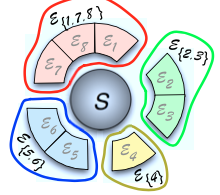
\includegraphics[width=0.6\textwidth]{2222.png}\hfill
   }
\end{center}
\caption{The figure illustrates the different fraction of the environment involved in the interaction with the quantum system composed of the signal part and the detector part.}
\label{111}
\end{figure}

For example, the photon comes out your thermal device, and your detector just come close to the device, and you only detector part of it but not all of it. And then, another specialty for us to define the environment separately is that because if we can only measure it once and the state will be destroyed to get turned into another state, then how come can we check if the signal which is measured is right? In this case, since the signal will leak to the some parts of the environment, so we can do checking doubly.\\

\subsection{The symmetry of the coherence and decoherence}
In another way to explain the decoherence phenomenon is to carry out the symmetry stuff in the same paper. If we just see the symmetry of the different state between the coherence region and decoherence region, you can find out that the tremendous different is that, for the phase of the coherence, the state could be the mixed up one since the exchanged law cant be applied at there in nature, resulting in the correction of describing the state with the wave in 0 to $2\pi$ as the example we gave before.( Not $2\pi$ necessary but the periodic physical parameters.) But when we just come to the entanglement part(Interact between the system and the environment) as the fig.\ref{8888} said, the information between the two system can exchange mathematically. On the other hand, the phase can't be the periodic since the they just mix up together. So in the end, we could end up figuring out the final state with the "wavepacket-collapse" by using the entanglement interpretation, and the system will turn into the localized state staying at the same state. \\
\begin{figure}
\begin{center}
   \subfigure[] {
   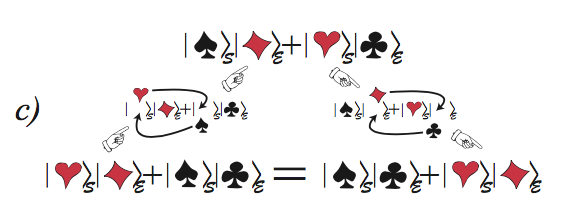
\includegraphics[width=0.6\textwidth]{8888.png}\hfill
   }
\end{center}
\caption{The figure illustrates the symmetry of transforming the information between the system and the environment. You can see that after the information from the left (in the quantum system) copy to the right (classical system), the information can be reserved as its original type. }
\label{8888}
\end{figure}

The case as there can be seen clearly in the example of the atom I've told in the previous section, when it just starts, it is in the state of the asymmetry, and we can't change the state as well, so we can lead out the coherence plot as the "superposition" case, but after the coherent time, which means the leverage between the system and the environment got balance, and everything is nailed down by the entanglement lead by the symmetry.\\

\subsection{The solutions to the puzzles}
So for the first puzzles on the non-intuitive superposition, I think the decoherence can totally explain this one as a "wave" superposition since it is very natural! Because when the wave is propagating, we can use many states to express the phase of this states, and it is reasonable, instead of just saying that the "possible states" combinations and no further instruction. For the second puzzles written in a way of speculating the reasonable of the collapse, since it just want to avoid the terrifying problem happening to the real quantum system actually including the tremendous non-measurable states and can't be figured out prefect.  In the way used by the decoherence, it applies the wave interacting with the environment and in the end it will get decoherence and stay at the certain level and won't change, and it is the beautiful way to solve the problem without adding the inexplicable suppose. At the end of the puzzles, actually this is the natural expression as you can see through the report, the wave which is used to say the superposition expressing in the decoherence.\\

Till now, we've been looking at the basic concepts of the decoherence and the way it solves the problem existing in the main-stream party in the quantum mechanism. And now, let us take a look at the works which has been working on corroborating the ideas written in this theory!

\section{Experiments and results of them} 
So far, the theory of the decoherence has been well-described as the other one more beautiful than the Copenhagen's point to acknowledge our quantum system. In this section, the experiments of the related ones upon the decoherence will be demonstrated to talk the incredibly displayed out demonstrations happening in the labs.

In this section, I would like to introduce the first paper\cite{Hackerm_ller_2004} I've read that is the obvious case in order to find out the phenomenon of the decoherence clearly.\\

The setup of the experiment is in the Fig.\ref{666} quoted by the paper. In the paper, it just implements the thermal emission, which lightening the laser blocking on the way which the particle is gonne go through, to be their approach to induce the environment into this quantum system. And for the intensity of the "entanglement", which means the intensity of the coupling between the particle and the outside environment, is outperformed with form of the power of the laser acting on the particle as it's going through the light.\\

\begin{figure}
\begin{center}
   \subfigure[] {
   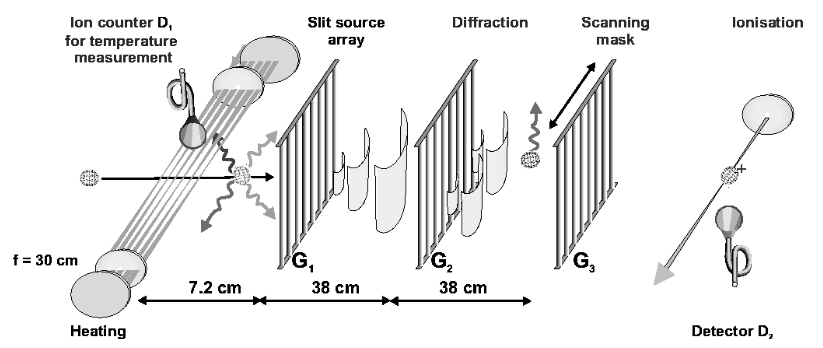
\includegraphics[width=0.8\textwidth]{6666.png}\hfill
   }
\end{center}
\caption{The figure illustrates setup of the experiment used in being the proof of the decoherence in the experiment of the thermal emission.}
\label{666}
\end{figure}

For these three gratings applied in the experiment, actually are the standard ones we usually use in the interference experiment. The first one is for the purpose of making the wave of going through the grating coherent again! And it is the normal SOP done on this kind of the experiment when executing on exploring the pattern of the diffraction/interference. And the second, demonstrably, is the one we adopt to have the wave diffracted for seeing some patterns. And in this experiment, it is used to see the pattern of that to see the wave and exam the suppose of the decoherence.  At the end of passing through the previous gratings, the grating for modulating the molecular density pattern is the necessary one installed in. And our measurement of the experiment is the ionization detector, which is applied to measure the wave acted on by the diffraction effect.\\

The significant results obtained from the paper are in the Fig.\ref{333}, which you can see the pattern clearly considerably. As you can see with the different power of the laser, the pattern of the wave is quiet different. From the smallest one, which is no laser applied case, can see the matter wave of the electron pretty well, is a beautiful wave as the one in the figure of the most left one. And then we make a decision of starting turning on the power of the laser, and you can see at first with the 3W, the pattern is a amplitude-amplified case as you can see because of the power is increased without the decoherence shows up. But when the power of it is getting higher and higher, and can see the the decline of the amplitude of the wave measured by our detector is getting smaller and smaller, and in the end, the you can see that the wave can't be demonstrated obviously and the phenomenon of the decoherence is well-looked.\\ 
\begin{figure}
\begin{center}
   \subfigure[] {
   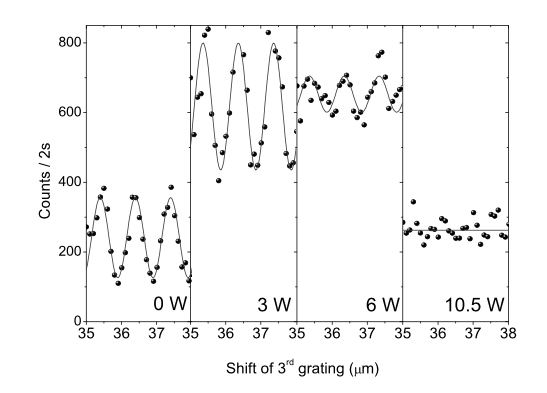
\includegraphics[width=0.6\textwidth]{3333.png}\hfill
   }
\end{center}
\caption{The figure illustrates that applying the different power of the laser refers to the various intensities of the environment-induced coupling. The three shifts used to see the transition clearly are the proof of the decoherence that the transition pattern can be obtained clearly.}
\label{333}
\end{figure}

For another picture digged out from the paper, the Fig.\ref{444} It indicates the fringe interference referred to the pattern of the decoherence is with respect to the power of laser clearly and a function of the temperature, directing to the laser power. You can see that in the lower power cases, the fringe is clear for us to see it as the coherence cases we could see with the "lower-interaction with the environment" case. But oppositely, after the certain threshold achieved in this case, the transition between the coherence(quantum) and the decoherence(classical) will be initiated.\\ 
\begin{figure}
\begin{center}
   \subfigure[] {
   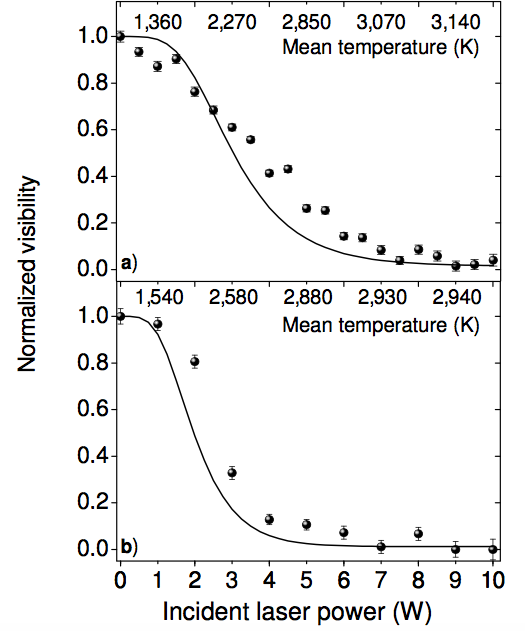
\includegraphics[width=0.6\textwidth]{4444.png}\hfill
   }
\end{center}
\caption{The figure illustrates the fringes as a function of the laser power representing the intensity of the interaction between the quantum system and the classical system. We can see the transition accompanying with the sharply crash down.}
\label{444}
\end{figure}

Stink to the same picture as the one in the previous paragraph, the one idea hits on my mind is why don't we find the inflection point of the line to be the significant point in the transition plot, and we can do some of the works on the point and see the sharp transition to see the boundary of the classical and quantum mechanism more clearly? More specific, if I take the lower picture as the example, and we can find something like 2.5W or similar, and we can just fix our power at there and do some works on minus and plus a little bit power on it. Then, we can try to prove some classical/quantum things in that special region, even test or define some properties with respect to the frame of the decoherence as a new party of the "Theory of everything." Just a guess but it appears to be an interesting question to me. )\\





\newpage
%%%%%%%%%%%%%%%%%%%%%% references %%%%%%%%%%%%%%%%%%%%%%%%%%%%%%
\section*{References}

\bibliographystyle{elsarticle-num}
\def\bibname{\Large\bf References}
\def\refname{\Large\bf References}
\pagestyle{plain}
\bibliography{biblio}



\end{document}
